\chapter{Applications to graph theory}

\section{The Azuma-Hoeffding Inequality}

\begin{definition}
    A sequence $X_0, \ldots, X_n$ of random variables is consider a \textbf{martingale} if, for every $i \leq n$,
    \[ \E [X_{i+1} | X_i,\ldots, X_0] = X_i \] 
\end{definition}

A random graph $G = G(n)$ is a graph that has $n$ labeled vertices and produces an edge between 2 of them with a probability. Let $v_1, \ldots, v_n$ denote the vertices of $G$ and $e_1, \ldots, e_m$ all of the $\binom{n}{2}$ potential edges that $G$ can produce. Also, define each edge's indicator function as it follows,
\[\1_{e_k \in G} = \begin{cases}
    1, & e_k \in G\\
    0, & \mbox{otherwise} 
\end{cases} \] 
An edge exposure martingale is a sequence of random variables defined as the expected value of a function $f(G)$ which depends on the information of the first $j$ potential edges:

\[ X_j = \E [f(G) \;|\; \1_{e_1 \in G}, \ldots, \1_{e_j \in G}] \] 

Since all of the graph information is contained in its edges, the sequence transitions from no information: $X_0 = E(f(G))$, to the true value of the function: $X_m = f(G)$. Similarly, one can define a martingale which depends on how many vertices are revealed. The vertex exposure martingale is defined as it follows,

\[ X_i = \E [f(G) \;|\; \1_{\{v_k, v_j\}\in G}, \; k < j \leq i] \] 

The following inequality is to some extend an adapted version of Hoeffding inequality~\ref{hoeffding:bounded} for martingale random variables. If we stablish a limit for which a martingale varies from one step to another, the theorem then states that we can exponentially bound the tails of its distribution:

%% --- Azuma's inequality
\begin{theorem}[Azuma-Hoeffding inequality]\label{azuma}
    Let $X_0, \ldots, X_m$ be a martingale with $X_0 = 0$, and
    \[ |X_{i+1} - X_i| \leq 1, \hspace*{1em} \forall i < m. \]
    Then, for $t > 0$,
    \[ \P\{X_m > t\sqrt{m}\} < e^{-t^2 / 2}. \] 
\end{theorem}

\begin{proof}
    First, we must prove another inequality.
    \begin{lemma}
        Let $Y_1, \ldots, Y_m$ be random variables such that $|Y_i| \leq 1$ and $\E Y_i = 0$, and let $S_m = \sum_{i = 1}^m Y_i$. Then, for $\lambda > 0$,
        \[ \E[e^{\lambda Y_i}] \;\leq\; e^{\lambda^2 / 2}. \]
    \end{lemma}

    \begin{proof}

    \begin{tabular}{cc}
        \(\displaystyle h(x) = \frac{e^\lambda + e^{-\lambda}}{2} + \frac{e^\lambda - e^{-\lambda}}{2} \cdot x,  \)
        &\hspace*{2em}
        \begin{tabular}[c]{@{}l@{}}
        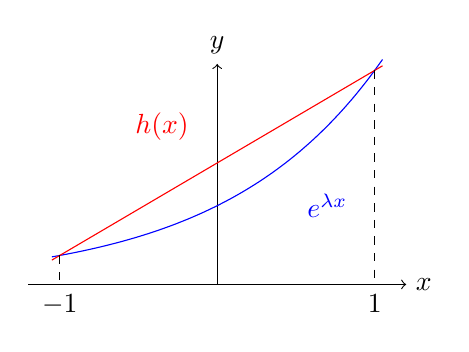
\begin{tikzpicture}
            \draw[->] (-2.4, 0) -- (2.4, 0) node[right] {$x$};
            \draw[->] (0, 0) -- (0, 2.8) node[above] {$y$};
            \draw[scale=1, domain=-2.1:2.1, smooth, variable=\x, blue] plot ({\x}, {e^(\x/2)});
            \draw[scale=1, domain=-2.1:2.1, smooth, variable=\y, red]  plot ({\y}, {(e+1/e)/2 + (e-1/e) * \y/4}); % Divided \x and \y by 2 on the 2nd coordinate to scale the y axis by 1/2.
                \node[text=red] at (-0.7,2) {$h(x)$};
            \node[text=blue] at (1.4,1) {$e^{\lambda x}$};
            \draw [dashed] (-2, {e^(-1)}) -- (-2,0)  node[below] {$-1$};
            \draw [dashed] (2, {e^(1)}) -- (2,0) node[below] {$1$};
        \end{tikzpicture} 
    \end{tabular}
    \end{tabular}

    As the picture above shows, $h(x)$ is the line that passes through the points $x = -1$ and $x = 1$ in the function $e^{\lambda x}$. Since $e^{\lambda x}$ is convex ($\lambda > 0$), it follows that $h(x) \geq e^{\lambda x} $ for $x \in [-1,1]$. Thus,

    \[\everymath{\displaystyle}\arraycolsep=1.8pt\def\arraystretch{1.8}
      \begin{array}{rcl}
        \E[e^{\lambda Y_i}] & \leq & \E[h(Y_i)] \\
        \text{\scriptsize ($h$ is linear)}& = & h(\E Y_i) = h(0)\\
        & = & \frac{e^\lambda + e^{-\lambda}}{2} = \cosh \lambda .
      \end{array}      
    \]
    Finally, $(2k)! \geq 2^k \cdot k! $, for every $k\in\N$. Thus,

    \[
        \E[e^{\lambda Y_i}]\leq \cosh \lambda \;=\; \sum_{k = 0}^\infty \frac{\lambda^{2k}}{(2k)!} \;\leq\; \sum_{k = 0}^\infty \frac{\lambda^{2k}}{2^k \cdot k!} \;=\; e^{\lambda^2 / 2}.
    \]

    \end{proof}

    Now, define $Y_i = X_i - X_{i-1}$. Then, by hypothesis, $|Y_i| \leq 1$ and
    \[ \E [Y_i | X_{i-1},\ldots, X_0] = \E [X_i - X_{i-1} | X_{i-1},\ldots, X_0] = X_i - X_i = 0. \] 
    Therefore, we can apply the previous inequality to assert,
    \[ \E [e^{\lambda Y_i} | X_{i-1},\ldots, X_0] \leq e^{\lambda^2/2}. \tag*{$ (\star) $}\]

    Using the formula $E[XY] = E_X [X E[Y|X]]$ we assert that
    \[ \E e^{\lambda X_m} \; = \;  \E\left[\prod_{i = 1}^{m-1} e^{\lambda Y_i} \cdot \E[e^{\lambda Y_m} | X_{m-1},\ldots, X_0]\right] \]

    We repeat this process $n$ times:
    \[ \everymath{\displaystyle}\arraycolsep=1.8pt\def\arraystretch{1.8}
        \begin{array}{r c c c l}
        & & \E e^{\lambda X_m}  =   \E \prod_{i = 1}^{m} e^{\lambda Y_i} \hfill\\
        & = & \E\left[\prod_{i = 1}^{m-1} e^{\lambda Y_i} \cdot \E[e^{\lambda Y_m} | X_{m-1},\ldots, X_0]\right] \hfill & \overset{(\star)}{\leq} & \E\left[\E \prod_{i = 1}^{m-1} e^{\lambda Y_i} \right] e^{\lambda^2 / 2}\\
        & = & \E\left[\prod_{i = 1}^{m-2} e^{\lambda Y_i} \cdot \E[e^{\lambda Y_{m-1}} | X_{m-2},\ldots, X_0]\right]e^{\lambda^2 / 2} & \overset{(\star)}{\leq} & \E\left[\E \prod_{i = 1}^{m-2} e^{\lambda Y_i} \right] e^{2\lambda^2 / 2}\\
        & = & \hfill\vdots\hfill & \leq & \hfill\vdots\hfill\\
        & = & \E\left[\E[e^{\lambda Y_{1}} |  X_0]\right]e^{\lambda^2 / 2} & \leq & \hfill e^{m\lambda^2/2} \hfill
    \end{array} \tag*{$ (*) $} \]
    At last, by setting $\lambda = t/\sqrt{m}$ we obtain,
    \[ \everymath{\displaystyle}\arraycolsep=1.8pt\def\arraystretch{1.8}
    \begin{array}{r c l}
        \P\{X_m > t\sqrt{m}\} & = & \P\{e^{\lambda X_m} > e^{\lambda t \sqrt{m}}\} \\
        \text{\scriptsize (Markov)}& \leq & \E[e^{\lambda X_m} ] e^{-\lambda t \sqrt{m}}\\
        & \overset{(*)}{\leq} & e^{m\lambda^2/2} \cdot e^{-\lambda t \sqrt{m}}\\
        \text{\scriptsize ($\lambda = t/\sqrt{m}$)} & = & e^{t^2/2} e^{-t^2} = e^{-t^2 / 2}.
    \end{array}    \tag*{$ (\bullet) $}
    \]
\end{proof}
%% --------------------

\begin{remark} We assumed that $X_0 = 0$ to lighten the notation. However, we can remove this restriction by replacing $X_m$ with $X_m - X_0$ in some crucial steps:
    \[\everymath{\displaystyle}\arraycolsep=1.8pt\def\arraystretch{1.8}
        \begin{array}{rl}
            & X_m-X_0 = \sum_{i = 1}^n Y_i\\
            \overset{(*)}{\implies} & \E e^{\lambda (X_m-X_0)} = \E \prod_{i = 1}^{m} e^{\lambda Y_i} \leq e^{m \lambda^2 / 2}\\
            \overset{(\bullet)}{\implies} & \P\{X_m-X_0 > t\sqrt{m}\} \leq e^{-t^2/2}
        \end{array} 
        \] 

\end{remark}    

In the following section we are going to present an application of the Azuma-Hoeffding inequality to prove the convergence to the mean of a fast (but not effective) approximation algorithm for the \textit{Travelling Salesman Problem}. 

\section{An heuristic algorithm for the Travelling Salesman Problem}

Let $X_1,\ldots, X_N$ be a sample of $N$ uniformly distributed points in a compact square $[0,L]\times [0,L]$. The algorithm divides this square in $M$ stripes of width $L/M$ each. Then, it connects each of the points in each of the stripes vertically and connects the top-most of one stripe with the top-most of the next one (or viceversa as the image below shows).

\begin{figure}[ht]\label{TSP:pic0}
    \centering
    \subfloat[Uniform sample]{\label{TSP:pic0.1}
        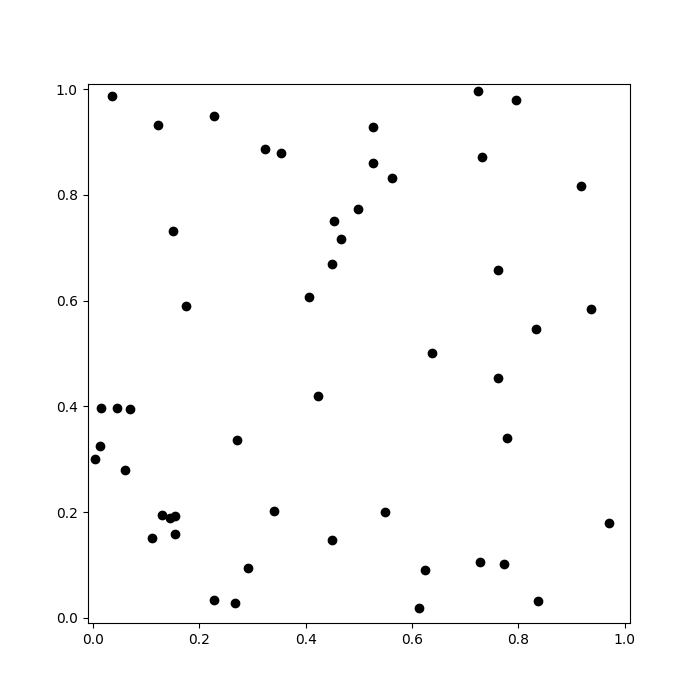
\includegraphics[width=0.33\textwidth]{../Simulation/TSPPictures/ex0.png}
    }
    \subfloat[Divide in $M$ stripes]{\label{TSP:pic0.2}
        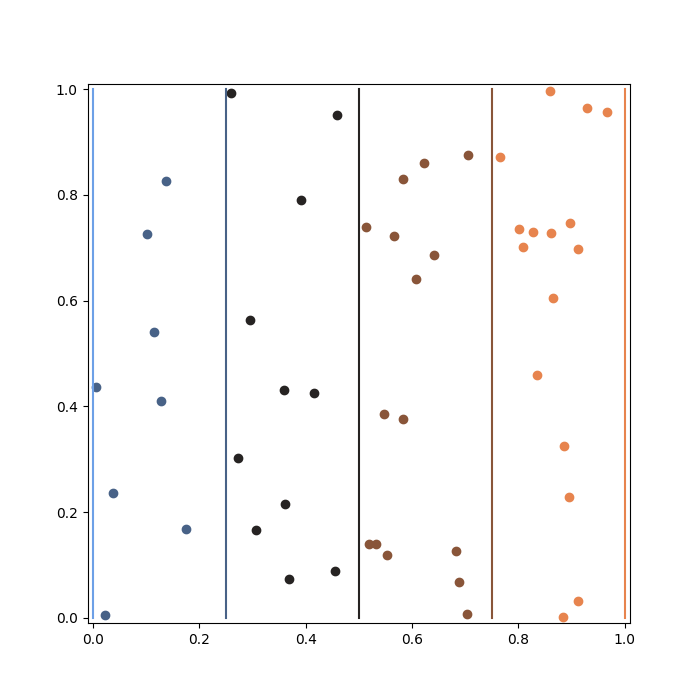
\includegraphics[width=0.33\textwidth]{../Simulation/TSPPictures/ex1.png}
    }
    \subfloat[Join points vertically]{\label{TSP:pic0.3}
        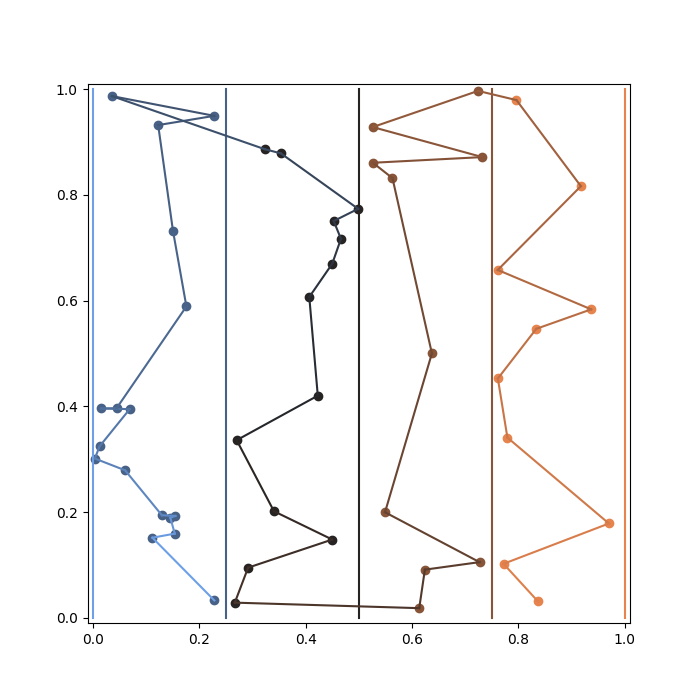
\includegraphics[width=0.33\textwidth]{../Simulation/TSPPictures/ex2.png}
    }
\end{figure}

In the paper~\cite{gzyl1990physicist} the authors found that the optimal  number of stripes is $M^* = \floor{0.58 N^{1/2}}$. If $t_N$ is the TSP solution distance for our sample and $d_N$ is the algorithm's answer with the optimal $M^*$, then the error is asymptotically:
\[  \frac{d_N-t_N}{t_N} \approx 0.23.\] 

The result that we are going to show is that $d_n$ is very concentrated around its mean. In order to prove this, some modifications must be made to the algorithm's trajectory. Let $e_N$ be the distance of a new trajectory that satisfies the following conditions:
\begin{itemize}
    \item For any empty stripe in the plane we sum the length of its diagonal $\sqrt{L^2+ L^2/M^2}$ and then it skips the empty stripe.
    \item When there are no empty stripes, $e_N = d_N$ 
\end{itemize}
 Since the probability that any given stripe is empty converges exponentially to 0,
\[ \begin{array}{rl}
    {(1- 1/M)}^N & = {(1- 0.58^{-1} N^{-1/2})}^N\\[1em]
    & = {\left({(1- 1/M)}^{M}\right)}^{0.58^{-1} N^{1/2}}\\[1em]
    &  \sim \exp(-0.58^{-1} N^{1/2}).
\end{array} \] 


Let $\A_i := \sigma\{X_1,\ldots,X_i\}$ denote the sigma algebra corresponding to revealing the first $i$ points, $\A_0 = \{\emptyset, {[0,L]}^2\}$. The expected value of the trajectory $e_N$ given that we only know the positions of the first $i$ points in the sample is $\E (e_N | \A_i)$. Define
\[ Z_i = \E (e_N | \A_i) - \E (e_N | \A_{i-1}),  \]  
As the difference of this expectations when we reveal 1 more point. Note that since
\[ \E(Z_i | \A_i) =  \E (e_N | \A_i, \A_i) - \E (e_N | \A_{i-1}, A_i) = \E (e_N | \A_i) - \E (e_N | \A_i) = 0,\] 
$Z_1, \ldots, Z_N$ is the difference sequence of a vertex exposure martingale.

\begin{figure}[ht]\label{TSP:pic1}
    \subfloat[$i = 0$]{\label{TSP:pic1.1}
        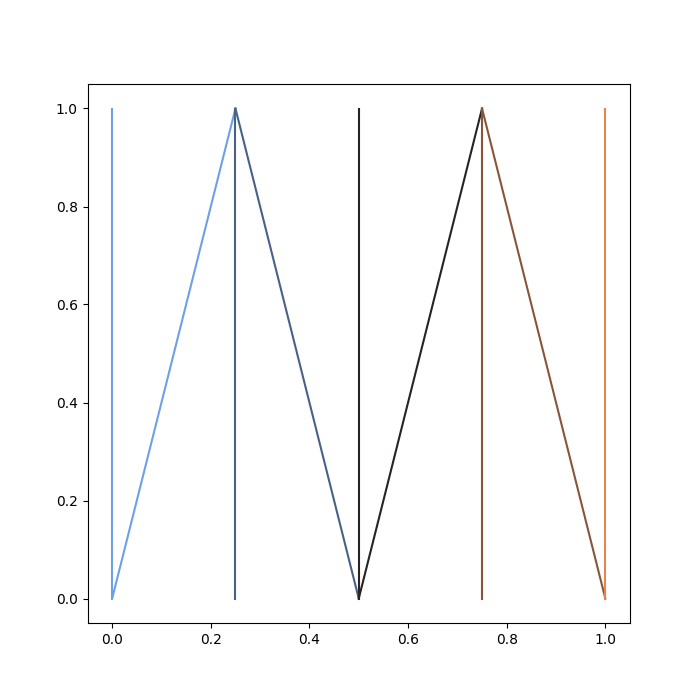
\includegraphics[width=0.25\textwidth]{../Simulation/TSPPictures/pic0.png}
    }
    \subfloat[$i = 1$]{\label{TSP:pic1.2}
        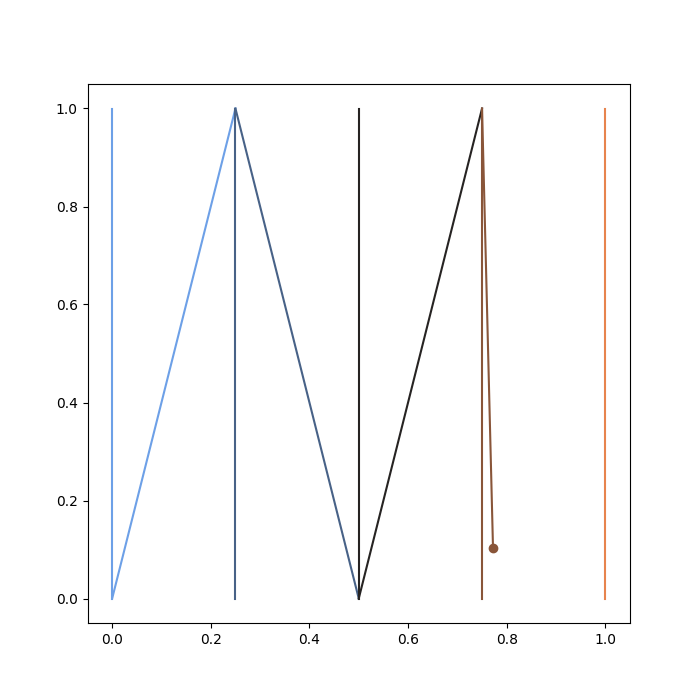
\includegraphics[width=0.25\textwidth]{../Simulation/TSPPictures/pic1.png}
    }
    \subfloat[$i = 2$]{\label{TSP:pic1.3}
        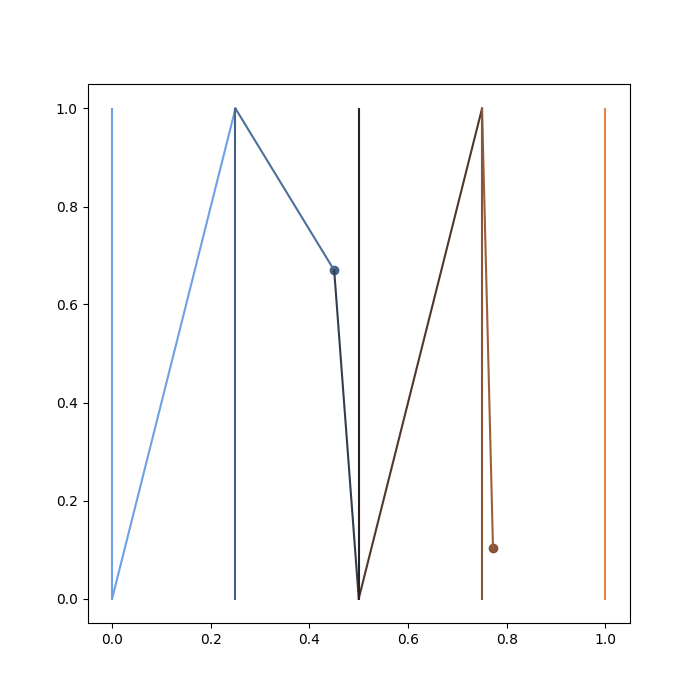
\includegraphics[width=0.25\textwidth]{../Simulation/TSPPictures/pic2.png}
    }
    \subfloat[$i = 4$]{\label{TSP:pic1.4}
        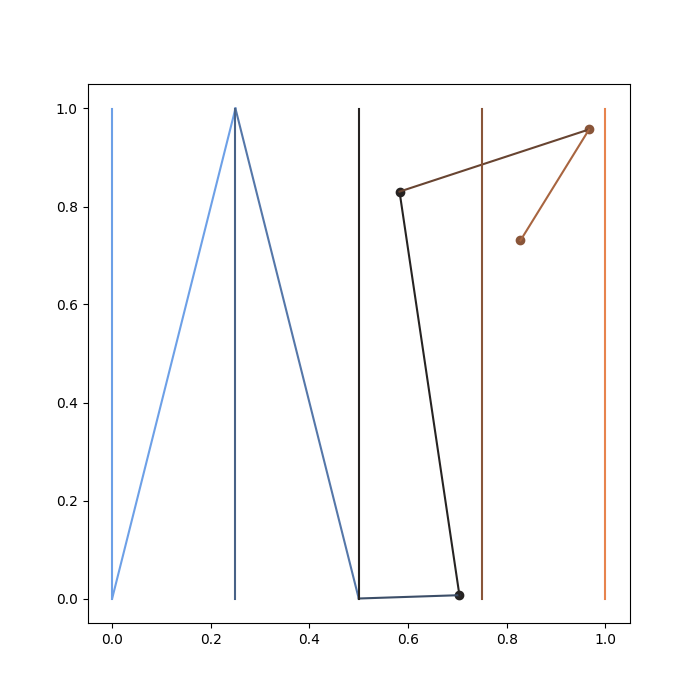
\includegraphics[width=0.25\textwidth]{../Simulation/TSPPictures/pic3.png}
    }

    \subfloat[$i = 7$]{\label{TSP:pic1.5}
        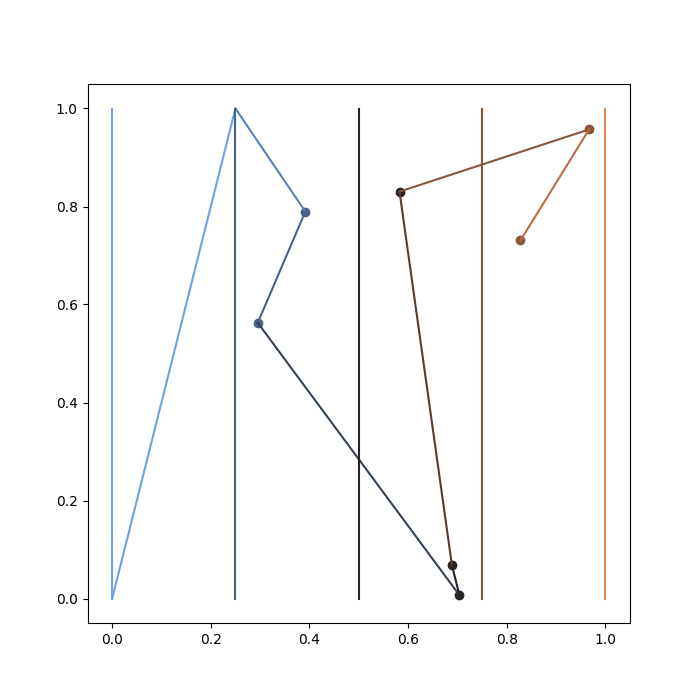
\includegraphics[width=0.25\textwidth]{../Simulation/TSPPictures/pic4.png}
    }
    \subfloat[$i = {12}$]{\label{TSP:pic1.6}
        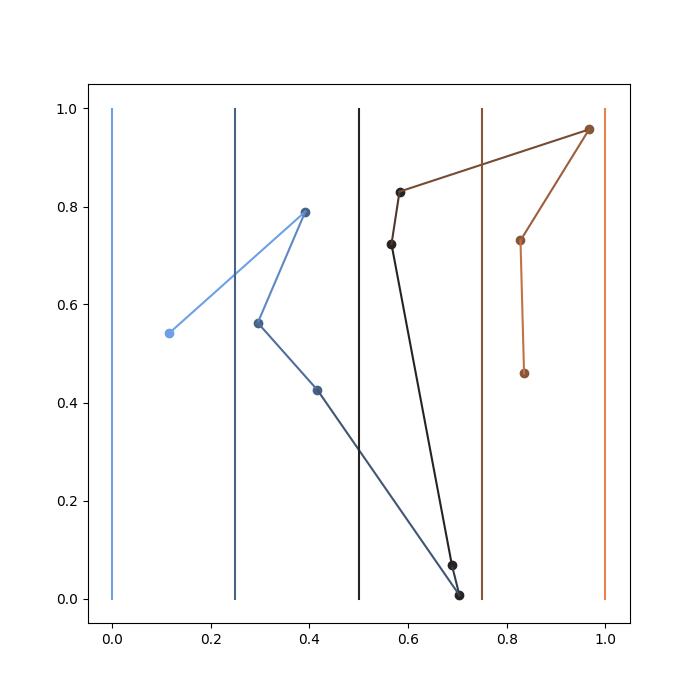
\includegraphics[width=0.25\textwidth]{../Simulation/TSPPictures/pic5.png}
    }
    \subfloat[$i = {18}$]{\label{TSP:pic1.7}
        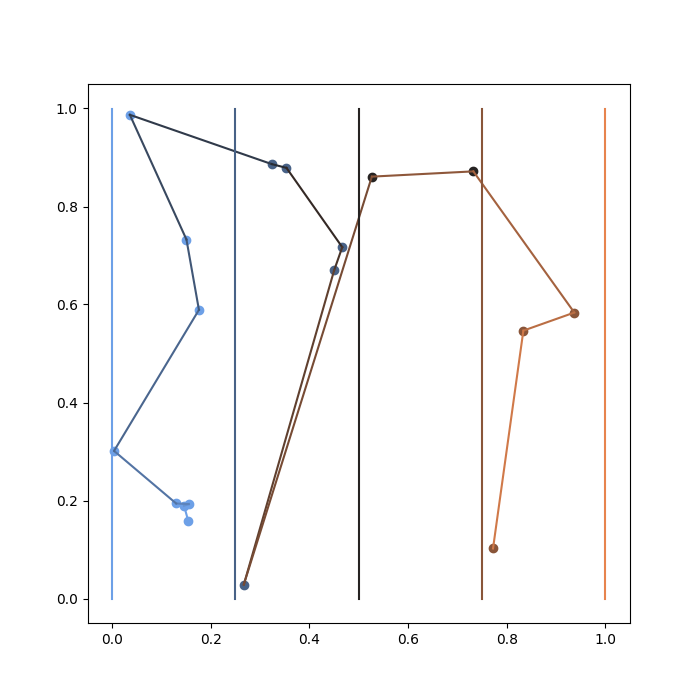
\includegraphics[width=0.25\textwidth]{../Simulation/TSPPictures/pic6.png}
    }
    \subfloat[$i = N = 50$]{\label{TSP:pic1.8}
        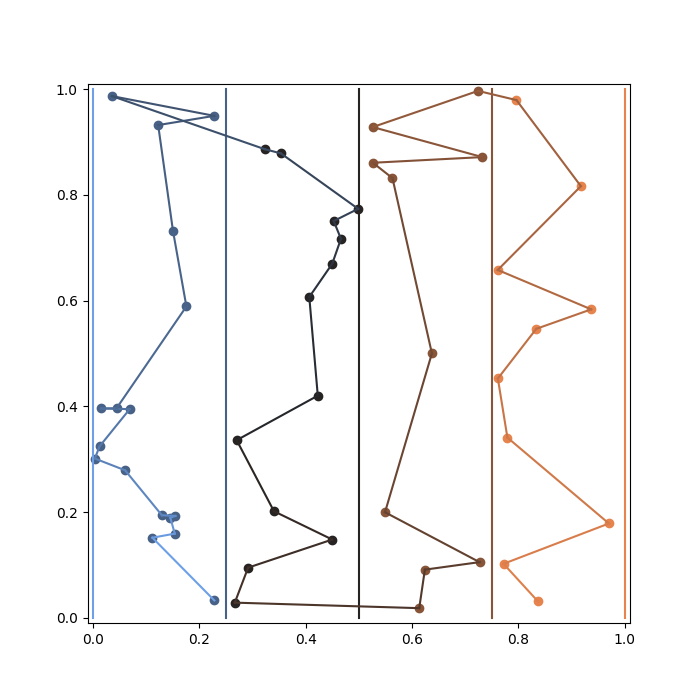
\includegraphics[width=0.25\textwidth]{../Simulation/TSPPictures/ex2.png}
    }
    \caption{Evolution of the vertex exposure martingale}
\end{figure}

Define $e_N^{[i]}$ as the distance of the trajectory when we remove the $i$-th point from the sample. Intuitively from the triangle inequality, we can obtain the following inequalities:
\[ e_N^{[i]} \leq e_N \leq e_N^{[i]} + 2 L/M, \]
meaning that revealing one point cannot increase more than 2 widths the distance of the trajectory. Thus,
\[ \|Z_i\|_\infty = \sup_{X_1,\ldots, X_N} \|\E (e_N | \A_i) - \E (e_N | \A_{i-1})\| \leq 2L/M. \tag*{$ (\star)$}.\]

On the other hand,
\[  e_N - \E e_N = \E (e_N | \A_N) - \E (e_N | \A_{0}) = \sum_{i = 1}^{N} Z_i.\]
Therefore, by the Azuma-Hoeffding inequality,
\[ \P \{ |e_N - \E e_N| > t \} \leq 2\exp\left(\frac{-t^2}{2}\sum_{i = 1}^{N} \|Z_i\|_{\infty}^2 \right). \] 
Finally,
\[ \sum_{i = 1}^{N} \|Z_i\|_{\infty}^2 \leq \frac{4NL^2}{M^2}, \]
which implies that
\[\P \{ |e_N - \E e_N| > t \} \leq 2\exp\left(\frac{-t^2}{2}\sum_{i = 1}^{N} \frac{4NL^2}{M^2} \right) \sim e^{-t^{2} K N}, \] 
for some $K\in \R^+$.

\section{Three additional short examples}

Three examples from~\cite{alon2016probabilistic} will be exposed to illustrate some ideas that can be associated with the main inequality of this chapter. Furthermore, the usefulness of the Azuma-Hoeffding inequality in the study of graphs and metric spaces can be used in a more general frame. Let $\Omega = A^B$ be the set of all functions $g: B\to A$ for which a probability measure is assigned
\[ \P\{g(b) = a\} = p(a,b),\hspace*{1em} \sum_{a\in A} p(a,b) = 1. \]
All the values $g(b)$ are mutually independent. Now, fix a chain of sets 
\[ \emptyset = B_0 \subset B_1 \subset \ldots \subset B_m = B,\hspace*{1em} \mathcal{B} = {\{B_i\}}_{i = 0}^m \]
and let $L: A^B \to \R$ be a functional. The martingale sequence $X_0,\ldots, X_m$ associated with $L$ and $\mathcal{B}$ is

\[ X_i(g) = \E[ L(g) \;|\; g(b),\; b\in B_i ] \] 

\begin{theorem}\label{lipschitz-condition}
    
\end{theorem}


Let $g \in {[n]}^{n}$ be a random vector (uniformly chosen) with $n$ entries, in which every entry is in $[n] = \{1,\ldots n\}$. Define $L(g)$ to be the amount of number that are not included in the vector,
\[ L(g) = \# \{ k \;:\; g_i \neq k,\; \forall i \in [n]\} = \sum_{k = 1}^{n} \1_{k \not\in g} \] 
For example,

\[ L(\underset{g_1}{1},\underset{g_2}{3},\underset{g_3}{1},\underset{g_4}{6},\underset{g_5}{4},\underset{g_6}{3}) = 2.\;\text{ (2 and 5 are missing)} \]

We can understand the process of choosing $g$ as independently assigning a random number in each of its coordinates. Thus, for a number $k \in [n]$, the probability of that number to not be in any of the entries of the vector is
\[\E \1_{k \not\in g} = \P\{g_i \neq k, \; \forall i\} = \prod_{i = 1}^n P\{g_i \neq k\} = {\left(1-\tfrac{1}{n}\right)}^n. \] 
Hence,
\[ \E L(g) = \sum_{k = 1}^n \P\{g_i \neq k, \; \forall i\} = n {\left(1-\tfrac{1}{n}\right)}^n \sim \frac{n}{e}. \] 
Now, define
\[\begin{array}{rcl}
    X_0(g) & = & \E L(g) \sim \frac{n}{e}\\
    X_1(g) & = & \E [ L(g) | g_1 ] \\
    \hfill\vdots\hfill & = & \vdots \\
    X_j(g) & = & \E [L(g) | g_1, \ldots, g_j ]\\
    \hfill\vdots\hfill & = & \vdots \\
    X_n(g) & = & \E [L(g) | g_1, \ldots, g_n] = L(g)
\end{array} \] 
$X_k(g)$ is the martingale that exposes one coordinate of $g$ at a time. The value of $L(g)$ can vary at most by 1 for each coordinate we reveal, so $L(g)$ has the Lipschitz condition. Then, we use \text{theorem}~\ref{lipschitz-condition} and Azuma-Hoeffding inequality to conclude that
\[ \P\{|L(g) - \tfrac{n}{e}| > t\sqrt{n}\} < 2e^{-t^2 / 2}. \] 



\vspace*{3em}
